\documentclass[10pt]{beamer}

\usepackage[T2A]{fontenc}
\usepackage[utf8]{inputenc}
\usepackage[russian,english]{babel}
\usepackage{subfig}
\usepackage[noend]{algorithm,algpseudocode}
\usepackage{amsmath}

\usepackage{booktabs}
\usepackage[scale=2]{ccicons}

\usepackage{pgfplots}
\usepgfplotslibrary{dateplot}

\usepackage{xspace}
\newcommand{\TODO}[1]{\textbf{\textcolor{red}{TODO: #1}}}


\algblockdefx{MRepeat}{EndRepeat}{\textbf{repeat}}{}
\algnotext{EndRepeat}

\algrenewcommand\alglinenumber[1]{\footnotesize #1}
\DeclareMathOperator{\rank}{rank}
\DeclareMathOperator{\sign}{sign}

\newcounter{mycounter}

\newcommand{\myparagraph}{\stepcounter{mycounter}\paragraph{\arabic{mycounter}}}

\newcommand{\xred}{\textcolor{red}{x}}
\newcommand{\xblue}{\textcolor{blue}{(X^l)}}
\newcommand{\blue}[1]{\textcolor{blue}{#1}}

\title{Лекция 11}
\subtitle{Анализ смещения и разброса}

\begin{document}

\section{Разбор летучки}

\maketitle

\begin{frame}{Постановка задачи}
  $X$ -- множество объектов \\
	$Y$ -- ответы в $\mathbb{R}$ \\
	Обучающая выборка: ${X^l = (x_i, y_i)_{i=1}^l}$ \\ 
	Целевая функция: $f: X \rightarrow Y$\\
	\bigbreak
	Набор моделей алгоритмов $A_t: X \rightarrow Y$, $t \in T$ \\
	Методы обучения $\mu: (X \times Y)^l \rightarrow A_t$, $t \in T$ \\
\end{frame}

\begin{frame}{Внешний функционал}  
  $$E_{in} = Q_{\mu}(X^l) = Q(\mu(X^l), X^l)$$\\
  \bigbreak
  Внешний функционал по отложенной выборке:\\
  $$E_{out} = Q_{\mu}(X^t, X^k) = Q(\mu(X^t), X^k)$$\\
\end{frame}

\begin{frame}{Линейная регрессия}  
  $$E_{in} = Q(w,X^l) = \sum\limits_{i=1}^l (f (x_i, w) - y_i)^2  = \Vert Xw - y \Vert^2 \rightarrow \min\limits_{w}$$
  \bigbreak
  Внешний функционал по отложенной выборке:\\
  $$E_{out} = Q(w^*,X^k) = \Vert X^k w^* - y \Vert^2$$
\end{frame}

\begin{frame}{Постановка задачи}
  \alert{Хотим}: $E_{out} \rightarrow \min $
  \bigbreak
  \pause
  $\vert A_t \vert \uparrow \quad \Rightarrow$ больше шансов, что целевая функция $f$ находится во множестве \\
  $\vert A_t \vert \downarrow \quad \Rightarrow$ лучше обобщающая способность алгоритма
\end{frame}

\begin{frame}{Постановка задачи}
  Ошибка алгоритма складывается из двух частей:
  \begin{itemize}
    \item Насколько хорошо $A_t$ может приблизить целевую функцию $f$
    \item Можем ли мы на основании $X^l$ выбрать $f$ из $A_t$
  \end{itemize}
\end{frame}

\begin{frame}{Внутренний функционал качества}
  Квадратичная функция потерь:\\
  $$L_i(a) = (a(x_i) - f(x_i))^2$$\\
  \bigbreak
  Внутренний функционал:
  $$E_{in} = \sum\limits_{i=1}^l (a(x_i, w) - f(x_i))^2 \rightarrow \min\limits_{w}$$
\end{frame}

\begin{frame}{Внешний функционал качества}
  $$E_{out}(a^{\xblue}) = \mathbb{E}_{\xred} \left[ (a^{\xblue}(\xred) - f(\xred))^2 \right] $$
  \bigbreak
  \pause
  \begin{align*} 
    \mathbb{E}_{\xblue} \left[ E_{out}(a^{\xblue}) \right] &= 
    \mathbb{E}_{\xblue} \left[ \mathbb{E}_{\xred} \left[ (a^{\xblue}(\xred) - f(\xred))^2 \right] \right]\\ 
    &= \mathbb{E}_{\xred} \left[ \mathbb{E}_{\xblue} \left[ (a^{\xblue}(\xred) - f(\xred))^2 \right] \right]
  \end{align*}  
\end{frame}

\begin{frame}{Средний метод}
  $$ \mathbb{E}_{\xblue} \left[ (a^{\xblue}(\xred) - f(\xred))^2 \right] $$
  \bigbreak \pause
  $$ \bar{a}(\xred) = \mathbb{E}_{\xblue} \left[ a^{\xblue}(\xred) \right] 
  \approx \frac{1}{K} \sum\limits_{k=1}^K a^{\blue{X_k}}(\xred)$$ \\
  \bigbreak
  $X_1, \dots, X_K$ -- различные обучающие выборки
\end{frame}

\begin{frame}{Средний метод}
  \(
    \mathbb{E}_{\xblue} \left[ (a^{\xblue}(\xred) - f(\xred))^2 \right] =
    \mathbb{E}_{\xblue} \left[ (a^{\xblue}(\xred) - \bar{a}(\xred) + \bar{a}(\xred) - f(\xred))^2 \right] 
  \)\\
  \pause
  \bigbreak
  \(
   \phantom{\mathbb{E}_{\xblue} \left[ (a^{\xblue}(\xred) - f(\xred))^2 \right]}  
    = \mathbb{E}_{\xblue} [ (a^{\xblue}(\xred) - \bar{a}(\xred))^2 + (\bar{a}(\xred) - f(\xred))^2 
  \)\\        
  \(
    \phantom{\mathbb{E}_{\xblue} \left[ (a^{\xblue}(\xred) - f(\xred))^2 \right]}
     + 2(a^{\xblue}(\xred) - \bar{a}(\xred))(\bar{a}(\xred) - f(\xred))  ] 
  \)\\
  \pause
  \bigbreak
  \(
   \phantom{\mathbb{E}_{\xblue} \left[ (a^{\xblue}(\xred) - f(\xred))^2 \right]}  
    = \mathbb{E}_{\xblue} \left[ (a^{\xblue}(\xred) - \bar{a}(\xred))^2 \right] + (\bar{a}(\xred) - f(\xred))^2
  \)
\end{frame}

{\foot{Bias, Variance}
\begin{frame}{Смещение и разброс}
  \( 
  \mathbb{E}_{\xblue} [ (a^{\xblue}(\xred) - f(\xred))^2 ] = 
  \underbrace{\mathbb{E}_{\xblue} [ (a^{\xblue}(\xred) - \bar{a}(\xred))^2 ]}_{var(\xred)} + \underbrace{(\bar{a}(\xred) - f(\xred))^2}_{bias(\xred)}
  \)
  \bigbreak
  \pause
  \(
  \mathbb{E}_{\xblue}[ E_{out}(a^{\xblue}) ]  = \mathbb{E}_{\xred} [ \mathbb{E}_{\xblue} [ (a^{\xblue}(\xred) - f(\xred))^2 ] ]
  \)\\
  \pause
  \bigbreak
  \(
    \phantom{\mathbb{E}_{\xblue}[ E_{out}(a^{\xblue}) ] }
    = \mathbb{E}_{\xred} [var(\xred) + bias(\xred)]
  \)
  \pause
  \bigbreak
  \(
    \phantom{\mathbb{E}_{\xblue}[ E_{out}(a^{\xblue}) ]}
    = var + bias
  \)
\end{frame}
}

\begin{frame}{Смещение и разброс}
  Смещение (bias) -- насколько сложное семейство моделей (средняя ошибка по всевозможным обучающим выборкам $X^l$)\\
  \bigbreak
  Разброс (variance) -- на сколько чувствителен алгоритм к изменению обучающей выборки (как отличается ошибка, если обучать модель на разных наборах данных)  
\end{frame}

\begin{frame}{Смещение и разброс}
  \centering
  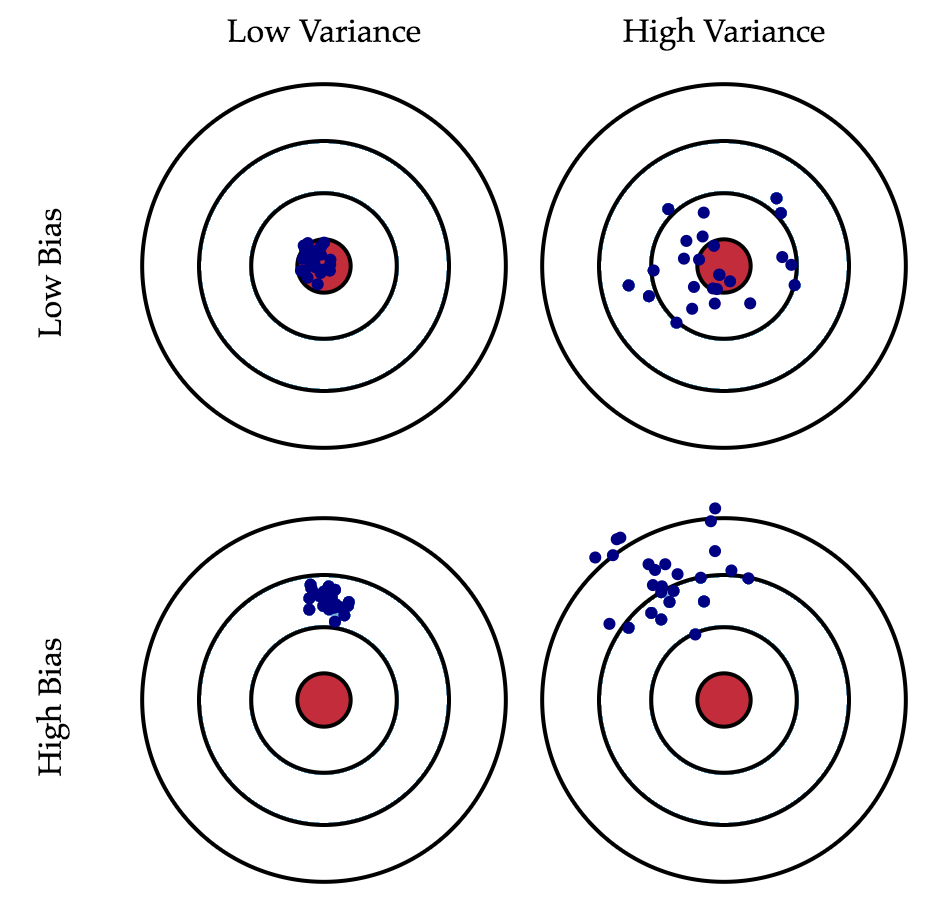
\includegraphics[width=0.8 \textwidth, height=0.8 \textheight,  keepaspectratio]{images/biasvariance}
\end{frame}

\begin{frame}{Смещение и разброс}
  Как правило, при увеличении сложности модели увеличивается разброс оценки, но уменьшается смещение.\\
  \bigbreak
  \pause
  Если же модель слабая, то она не состоянии выучить закономерность, в результате выучивается что-то другое, смещенное относительно правильного решения.
\end{frame}

%\begin{frame}{Пример}
%  \centering
%  \begin{minipage}[b]{.45\textwidth}
%    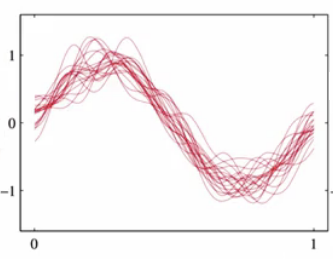
\includegraphics[width=\textwidth, keepaspectratio]{images/example2} 
%  \end{minipage}\qquad
%  \begin{minipage}[b]{.45\textwidth}
%    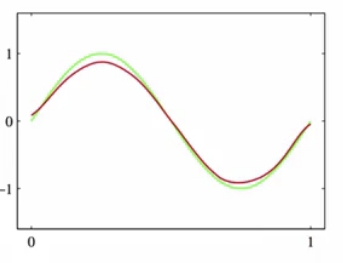
\includegraphics[width=\textwidth, keepaspectratio]{images/example1}
%  \end{minipage}
%\end{frame}

\begin{frame}{Пример $\sin$}
  \centering
  \begin{minipage}[b]{.45\textwidth}
    $f(x) = \sin (\pi x)$\\
    Количество объектов $l = 2$\\
    \bigbreak 
    Рассмотрим 2 модели:\\

      $A_1: h(x) = b$\\
      $A_2: h(x) = ax + b$

  \end{minipage}\qquad
  \begin{minipage}[b]{.45\textwidth}
    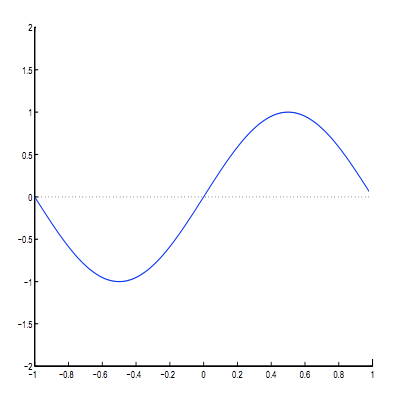
\includegraphics[width=\textwidth, keepaspectratio]{images/sin0}
  \end{minipage}
\end{frame}

\begin{frame}{Пример $\sin$}
  \centering
  \begin{minipage}[b]{.45\textwidth}
    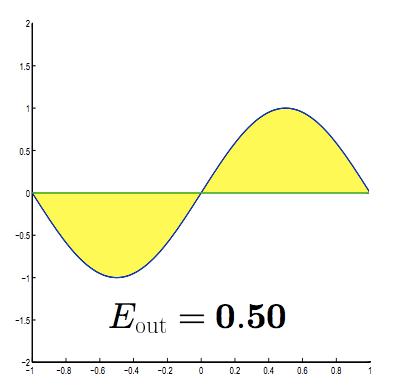
\includegraphics[width=\textwidth, keepaspectratio]{images/sin1} \\
    $$A_1$$
  \end{minipage}\qquad
  \pause
  \begin{minipage}[b]{.45\textwidth}
    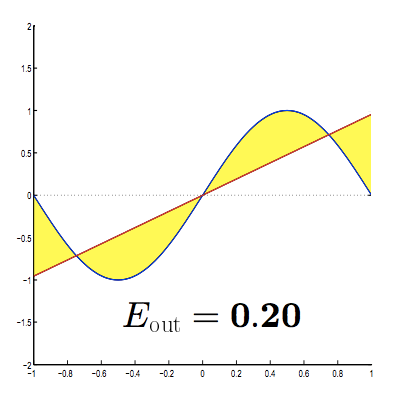
\includegraphics[width=\textwidth, keepaspectratio]{images/sin11}
    $$A_2$$
  \end{minipage}
\end{frame}

\begin{frame}{Обучение $A_1$, $A_2$}
  \centering
  \begin{minipage}[b]{.45\textwidth}
    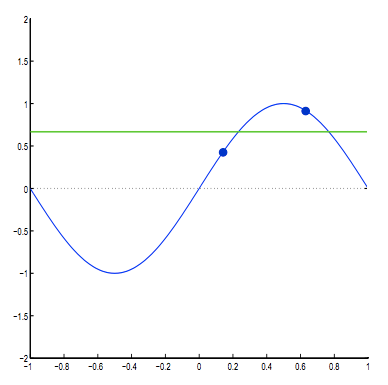
\includegraphics[width=\textwidth, keepaspectratio]{images/sin2} 
    $$A_1$$
  \end{minipage}\qquad
  \pause
  \begin{minipage}[b]{.45\textwidth}
    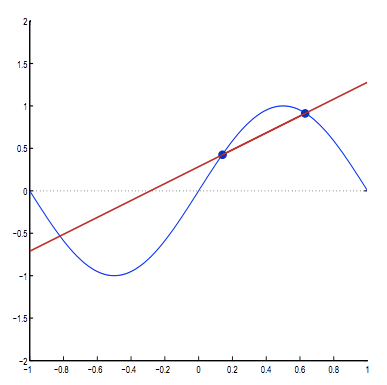
\includegraphics[width=\textwidth, keepaspectratio]{images/sin21}
    $$A_2$$
  \end{minipage}
\end{frame}

\begin{frame}{Bias-variance $A_1$}
  \centering
  \begin{minipage}[b]{.45\textwidth}
    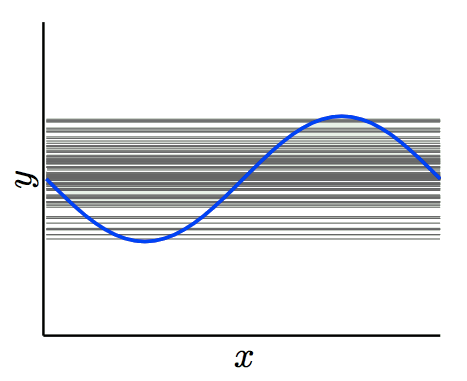
\includegraphics[width=\textwidth, keepaspectratio]{images/sin3} 
  \end{minipage}\qquad
  \pause
  \begin{minipage}[b]{.45\textwidth}
    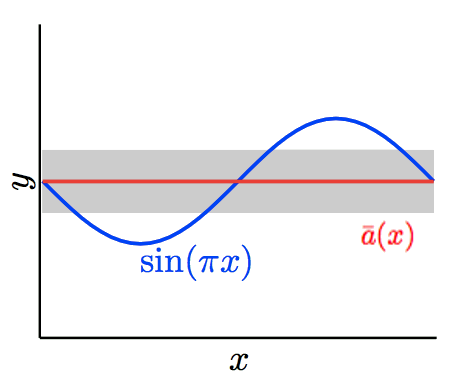
\includegraphics[width=\textwidth, keepaspectratio]{images/sin31}
  \end{minipage}
\end{frame}

\begin{frame}{Bias-variance $A_2$}
  \centering
  \begin{minipage}[b]{.45\textwidth}
    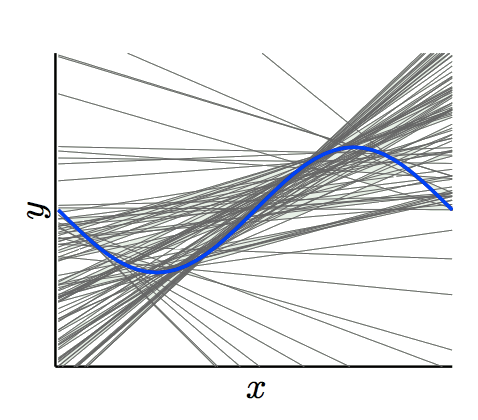
\includegraphics[width=\textwidth, keepaspectratio]{images/sin4} 
  \end{minipage}\qquad
  \pause
  \begin{minipage}[b]{.45\textwidth}
    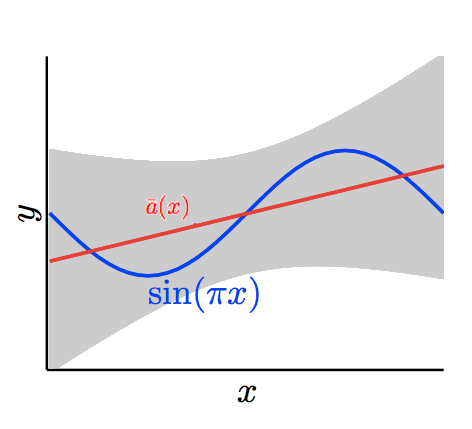
\includegraphics[width=\textwidth, keepaspectratio]{images/sin41}
  \end{minipage}
\end{frame}

\begin{frame}{Bias-variance }
  \centering
  \begin{minipage}[b]{.45\textwidth}
    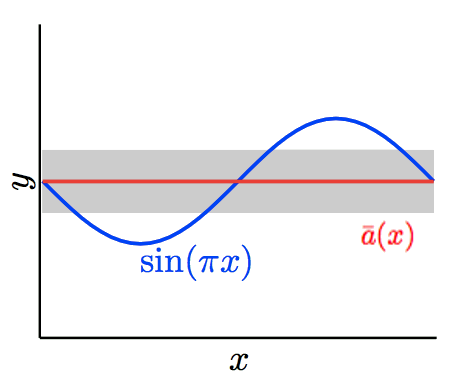
\includegraphics[width=\textwidth, keepaspectratio]{images/sin31} \\
    \centering
    bias = 0.50 \qquad var = 0.25
  \end{minipage}\qquad
  \pause
  \begin{minipage}[b]{.45\textwidth}
    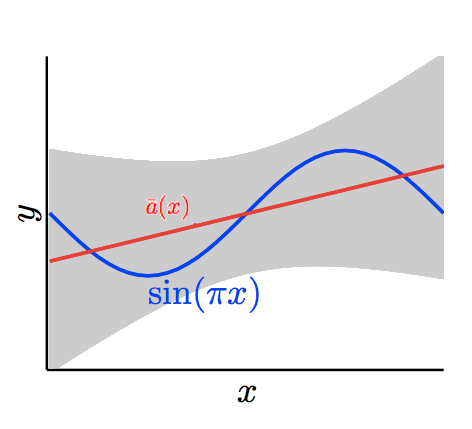
\includegraphics[width=\textwidth, keepaspectratio]{images/sin41}\\
    \centering
    bias = 0.21 \qquad var = 1.69
  \end{minipage}
\end{frame}

\begin{frame}{Мораль}
  Сложность модели нужно выбирать исходя из доступных данных, а не из предполагаемой сложности целевой функции.
\end{frame}
%
%\begin{frame}{Линейные модели}
%  Смещение может быть большим.\\
%  \bigbreak
%  Низкий разброс
%\end{frame}
%
%\begin{frame}{Деревья решений}
%  Низкое смещение \\
%  \bigbreak
%  Большой разброс
%\end{frame}

\section{Кривые обучения}

\begin{frame}{Матожидание $E_{in}$ и $E_{out}$}
  $$\mathbb{E}_{\xblue} \left[ E_{out}(a^{\xblue}) \right] $$\\
  \bigbreak \pause
  $$\mathbb{E}_{\xblue} \left[ E_{in}(a^{\xblue}) \right] $$\\
  \bigbreak \pause
  Как зависят от длины выборки?
\end{frame}

\begin{frame}{Простая модель}
  \centering
  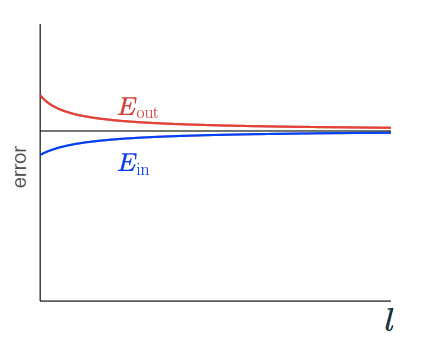
\includegraphics[width=0.8 \textwidth, keepaspectratio]{images/simple_model}
\end{frame}

\begin{frame}{High bias}
  \centering
  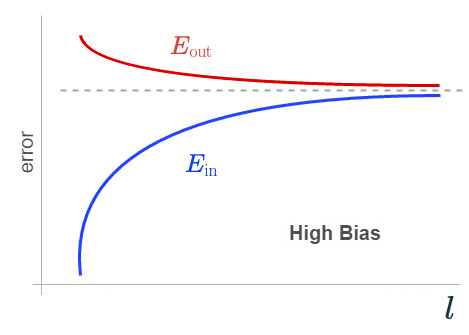
\includegraphics[width=0.8 \textwidth, keepaspectratio]{images/high_bias}
\end{frame}

\begin{frame}{Сложная модель}
  \centering
  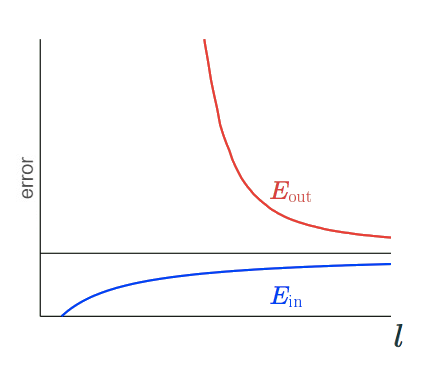
\includegraphics[width=0.8 \textwidth, keepaspectratio]{images/complex_model}
\end{frame}

\begin{frame}{High variance}
  \centering
  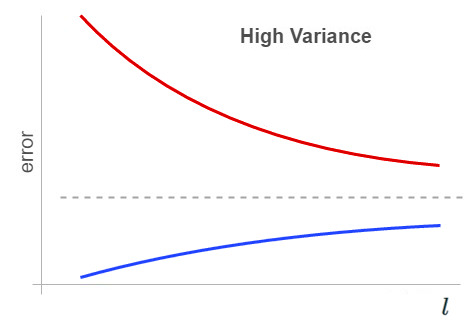
\includegraphics[width=0.8 \textwidth, keepaspectratio]{images/high_variance}
\end{frame}

\begin{frame}[standout]
  Вопросы?
\end{frame}

\appendix

\begin{frame}\frametitle{Что почитать по этой лекции}
  \begin{itemize}
    \item \href{http://work.caltech.edu/telecourse.html}{Professor Yaser Abu-Mostafa MOOC}
    \item  Hastie, T., Tibshirani R. "The Elements of Statistical Learning" Chapter 7 
  \end{itemize}
\end{frame}

\begin{frame}\frametitle{На следующей лекции}
	\begin{itemize}
    	\item[--] Методы восстановления регрессии
    	\item[--] K neighbors regressor 	    	
    	\item[--] Decision tree regression 
    	\item[--] Neural Net Regression
    	\item[--] SVR
	\end{itemize}
\end{frame}

\end{document}
